\documentclass[a4paper]{amsart}

\usepackage{color}
\usepackage[colorlinks=true, citecolor=red]{hyperref}  %needs to come before amsrefs package to work with \cite{}*{}
\usepackage{amssymb,latexsym}
\usepackage[alphabetic]{amsrefs}
\usepackage[mathscr]{eucal}
\usepackage{pdfsync}
\usepackage{graphicx}
\usepackage{epstopdf}
\DeclareGraphicsRule{.tif}{png}{.png}{`convert #1 `dirname #1`/`basename #1 .tif`.png}
\usepackage[all]{xy}
\usepackage{titletoc}
\usepackage{txfonts}   %  \fint  for integral average

%\usepackage{showkeys}  %options notref  notcite 

%\input{rgb.tex}

%\textcolor{DarkRed}{text in DarkRed}


\CompileMatrices

\theoremstyle{plain}
\newtheorem{theorem}{Theorem}[section]
\newtheorem{lemma}[theorem]{Lemma}
\newtheorem{proposition}[theorem]{Proposition}
\newtheorem{corollary}[theorem]{Corollary}

\theoremstyle{definition}
\newtheorem{definition}[theorem]{Definition}%[section]


\theoremstyle{remark}
\newtheorem{defn}[theorem]{Definition} 
\newtheorem{example}[theorem]{Example}
\newtheorem{remark}[theorem]{Remark}
\newtheorem{discussion}[theorem]{Discussion}

%\numberwithin{equation}{section}

%\newcommand{\abs}[1]{\lvert#1\rvert}

\DeclareMathOperator{\Lip}{Lip}
\DeclareMathOperator{\dist}{dist}
\DeclareMathOperator{\expected}{\mathbb{E}}
\DeclareMathOperator{\prb}{Prob}
\DeclareMathOperator{\spt}{spt}
\DeclareMathOperator{\lap}{\Delta}
\DeclareMathOperator{\Tr}{Tr}

\raggedbottom

\addtolength{\textwidth}{2cm}
\addtolength{\oddsidemargin}{-1cm}
\addtolength{\evensidemargin}{-1cm} 
\addtolength{\topmargin}{-1cm} 
\addtolength{\textheight}{2cm}

 
%%% BEGIN DOCUMENT
\begin{document}

\title{Beta Expansion}  
\author{John E.\ Hutchinson}
\date{\today}

%\begin{abstract} 
%This is the abstract
%\end{abstract}

\maketitle

%\tableofcontents


 \begin{figure}[htbp] %  figure placement: here, top, bottom, or page
    \centering
    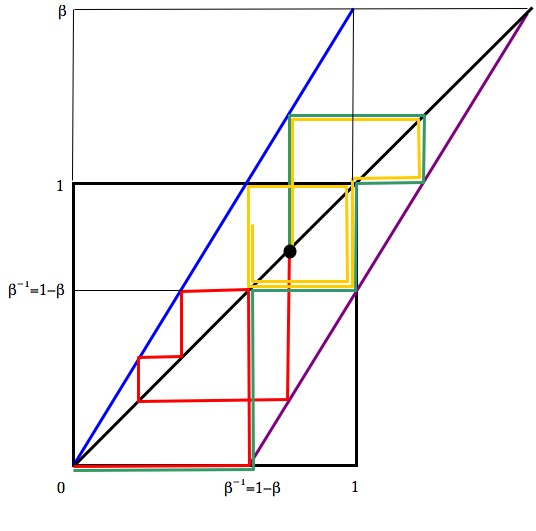
\includegraphics[width=5in]{beta.jpg} 
    \caption{Beta expansions of the golden mean.}
    \label{beta}
 \end{figure}
 
 
 
In the diagram, $ \beta = (1+\sqrt{5})/2\approx 1.618 $ satisfies  $ \beta ^2 - \beta = 1 = 0 $ and is the golden mean.

The black dot  is the point $ x = 3-\sqrt{5} \approx .764 $. Three $ \beta $-expansions of $ x $  are shown.

\begin{enumerate}

\item The red expansion is the \emph{greedy} expansion and gives
\[
x = \beta ^{-1} + \beta ^{-4} = 10010^\omega .
\]

\item The green expansion gives
\[
x = \beta ^{-2} + \beta ^{-3} + \beta ^{-4} = 01110^\omega .
\]
\item The yellow expansion is the \emph{lazy} expansion and gives
\[
x = \beta ^{-2} + \beta ^{-3} + \beta ^{-4} = 100(01)^\omega .
\] 
\end{enumerate} 

\newpage
\noindent \emph{Remarks}:
\begin{enumerate}
 \item From any $ x  \in [0,1)$ on the diagonal, one moves vertically to either the blue or violet line corresponding to the lines of slope $ \beta $ through $ 0 $ and $ \beta$ on the $ x $-axis.

Then move horizontally to the diagonal.   This gives $  T(x) $.  

\item For the greedy expansion one always stays in the  box $  [0,1)\times [0,1) $ and there is a unique choice of vertical move.  Equivalently, for $ x \in [0,1) $ one chooses
\[
 a(x)  = [\beta x ] , \quad T(x) = (\beta x ) = \beta x -  [\beta x ] .
 \]

\item For other allowable expansions note   the diagonal and  the crimson line cross at $ x= \beta $, and in general when
\[ 
x = \beta \left( x - [\beta ]\, \beta ^{-1} \right),\quad   \text{i.e.\ } x = \frac {[\beta ]}{\beta -1 }.
\]
 From geometric considerations the allowable values of $ a(x) $ are those integers such that
\[
0 \leq \beta - a(x) \leq \frac {[\beta ]}{\beta -1 }.
\]
%(One needs to slide the blue line $ x \mapsto \beta x $ down by an integer amount so that it is on or below the level $\dfrac {[\beta ]}{\beta -1 }$.   We allow  the greedy ``expansion''  of $\dfrac {[\beta ]}{\beta -1 }$ by taking an ``infinite number of steps'' down the crimson line.)
(One needs to slide the blue line $ x \mapsto \beta x $ down by an integer amount so that it is   below the level $\dfrac {[\beta ]}{\beta -1 }$.)
That is
\begin{align*}
\beta x -\frac {[\beta ]}{\beta -1 } &< a(x) \leq \beta x ,\\
\left[\beta x -\frac {[\beta ]}{\beta -1 }\right] + 1  &\leq  a(x) \leq [\beta x] .
\end{align*} 
 (C.f.\ [Barat et al\., p2003 (2)).  Note that if $ \beta $ is not an integer then $ [ \beta ] = \lceil \beta \rceil $ 
and note that ``$ \lceil $'' and ``$ \rceil $'' are used in the above reference.)

The value of $ T(x) $ is then 
\[ T(x) =  \beta x - a(x) ,
\]
which may be greater than $ 1 $.

\item For a proof of the Parry characterisation of the $ d\beta$-shift see~\cite{Fro}*{Theorem 7.2.9, p211}  (under Frougny, Numerations Systems, in my "Papers" collection). 
 
\end{enumerate} 

%%%%%%%%%%%%%%%%%%%%%%%%%%%%%%%%
%%%%%%%%%%%%%%%%%%%%%%%%%%%%%%%%
%%%%%%%%%%%%%%%%%%%%%%%%%%%%%%%%
%%%%%%%%%%%%%%%%%%%%%%%%%%%%%%%%
%\section{\textbf{Introduction}} 


 
 


 




%%%%%%%%%%%%%%%%%%%%%%%%%%%%%%%%
%%%%%%%%%%%%%%%%%%%%%%%%%%%%%%%%
%%%%%%%%%%%%%%%%%%%%%%%%%%%%%%%%
%%%%%%%%%%%%%%%%%%%%%%%%%%%%%%%%


\begin{thebibliography}{9} 

\bib{Fro}{book}{
   author={Lothaire, M.},
   title={Algebraic combinatorics on words},
   series={Encyclopedia of Mathematics and its Applications},
   volume={90},
   note={A collective work by Jean Berstel, Dominique Perrin, Patrice
   Seebold, Julien Cassaigne, Aldo De Luca, Steffano Varricchio, Alain
   Lascoux, Bernard Leclerc, Jean-Yves Thibon, Veronique Bruyere, Christiane
   Frougny, Filippo Mignosi, Antonio Restivo, Christophe Reutenauer,
   Dominique Foata, Guo-Niu Han, Jacques Desarmenien, Volker Diekert, Tero
   Harju, Juhani Karhumaki and Wojciech Plandowski;
   With a preface by Berstel and Perrin},
   publisher={Cambridge University Press},
%   place={Cambridge},
   date={2002},
   pages={xiv+504},
%   isbn={0-521-81220-8},
%   review={\MR{1905123 (2003i:68115)}},
}


\end{thebibliography}

\end{document} 

